\documentclass{beamer}
\usepackage[utf8]{inputenc}

\usetheme{Madrid}
\usecolortheme{default}
\usepackage{amsmath,amssymb,amsfonts,amsthm}
\usepackage{txfonts}
\usepackage{tkz-euclide}
\usepackage{listings}
\usepackage{adjustbox}
\usepackage{array}
\usepackage{tabularx}
\usepackage{gvv}
\usepackage{lmodern}
\usepackage{circuitikz}
\usepackage{tikz}
\usepackage{graphicx}

\setbeamertemplate{page number in head/foot}[totalframenumber]

\usepackage{tcolorbox}
\tcbuselibrary{minted,breakable,xparse,skins}



\definecolor{bg}{gray}{0.95}
\DeclareTCBListing{mintedbox}{O{}m!O{}}{%
  breakable=true,
  listing engine=minted,
  listing only,
  minted language=#2,
  minted style=default,
  minted options={%
    linenos,
    gobble=0,
    breaklines=true,
    breakafter=,,
    fontsize=\small,
    numbersep=8pt,
    #1},
  boxsep=0pt,
  left skip=0pt,
  right skip=0pt,
  left=25pt,
  right=0pt,
  top=3pt,
  bottom=3pt,
  arc=5pt,
  leftrule=0pt,
  rightrule=0pt,
  bottomrule=2pt,

  colback=bg,
  colframe=orange!70,
  enhanced,
  overlay={%
    \begin{tcbclipinterior}
    \fill[orange!20!white] (frame.south west) rectangle ([xshift=20pt]frame.north west);
    \end{tcbclipinterior}},
  #3,
}
\lstset{
    language=C,
    basicstyle=\ttfamily\small,
    keywordstyle=\color{blue},
    stringstyle=\color{orange},
    commentstyle=\color{green!60!black},
    numbers=left,
    numberstyle=\tiny\color{gray},
    breaklines=true,
    showstringspaces=false,
}
%------------------------------------------------------------
%This block of code defines the information to appear in the
%Title page
\title %optional
{5.4.23}
\date{september 2025}
%\subtitle{A short story}

\author % (optional)
{J.NAVYASRI- EE25BTECH11028}


\begin{document}

\frame{\titlepage}
\begin{frame}{Question:}
Using elementary transformations, find the inverse of the following matrix:
\[
A = \myvec{2 & -3 \\ -1 & 2}
\]

\end{frame}
\begin{frame}{Solution:}
We want to find the inverse of the matrix
\[
A = \myvec{2 & -3 \\ -1 & 2}.
\]

\textbf{Step 1: Assume the inverse matrix}

Let
\begin{equation}
A^{-1} = \myvec{x & y \\ z & w}
\end{equation}

By definition of inverse, we have
\begin{equation}
A A^{-1} = I = \myvec{1 & 0 \\ 0 & 1}
\end{equation}
\end{frame}
\begin{frame}{Solution:}
\textbf{Step 2: Multiply the matrices}

\begin{equation}
\myvec{2 & -3 \\ -1 & 2} \myvec{x & y \\ z & w} =
\myvec{2x - 3z & 2y - 3w \\ -x + 2z & -y + 2w}
\end{equation}

\begin{equation}
\myvec{2x - 3z & 2y - 3w \\ -x + 2z & -y + 2w} = 
\myvec{1 & 0 \\ 0 & 1}
\end{equation}

From this multiplication, we get the following system of equations:

\begin{equation}
2x - 3z = 1
\end{equation}

\begin{equation}
2y - 3w = 0
\end{equation}
\end{frame}
\begin{frame}{Solution:}
\begin{equation}
-x + 2z = 0
\end{equation}

\begin{equation}
-y + 2w = 1
\end{equation}

\textbf{Step 3: Solve the equations}

From equation (7):
\begin{equation}
-x + 2z = 0 \Rightarrow x = 2z
\end{equation}

Substitute into equation (5):
\begin{equation}
2(2z) - 3z = 1 \Rightarrow 4z - 3z = 1 \Rightarrow z = 1
\end{equation}

Then,
\begin{equation}
x = 2z = 2
\end{equation}
\end{frame}
\begin{frame}{Solution:}
From equation (8):
\begin{equation}
-y + 2w = 1 \Rightarrow y = 2w - 1
\end{equation}

Substitute into equation (6):
\begin{equation}
2(2w - 1) - 3w = 0 \Rightarrow 4w - 2 - 3w = 0 \Rightarrow w = 2
\end{equation}

Then,
\begin{equation}
y = 2w - 1 = 3
\end{equation}

\textbf{Step 4: Write the inverse matrix}

\begin{equation}
A^{-1} = \myvec{2 & 3 \\ 1 & 2}
\end{equation}

\end{frame}

\begin{frame}[fragile]
    \frametitle{Python Code}
    \begin{lstlisting}
import numpy as np
import matplotlib.pyplot as plt

# Define matrix A and its inverse
A = np.array([[2, -3],
              [-1, 2]])
A_inv = np.array([[2, 3],
                  [1, 2]])

# Define unit square vertices
square = np.array([[0, 0],
                   [1, 0],
                   [1, 1],
                   [0, 1],
                   [0, 0]])  # closed polygon
\end{lstlisting}
\end{frame}


\begin{frame}[fragile]
    \frametitle{Python Code}
    \begin{lstlisting}
# Apply transformations
square_A = square @ A.T
square_Ainv = square @ A_inv.T

# Plotting
plt.figure(figsize=(7, 7))
plt.plot(square[:,0], square[:,1], 'k--', label="Original Square")
plt.plot(square_A[:,0], square_A[:,1], 'r-', label="Transformed by A")
plt.plot(square_Ainv[:,0], square_Ainv[:,1], 'b-', label="Transformed by A⁻¹")
\end{lstlisting}
\end{frame}


\begin{frame}[fragile]
    \frametitle{Python Code}
    \begin{lstlisting}
# Style
plt.axhline(0, color='gray', lw=0.5)
plt.axvline(0, color='gray', lw=0.5)
plt.gca().set_aspect('equal', adjustable='box')
plt.legend()
plt.title("Effect of Matrix A and its Inverse on the Unit Square")
plt.grid(True)
plt.savefig("fig11.png")
plt.show()
\end{lstlisting}
\end{frame}

\begin{frame}{Plot-Using by Python}
    \centering
    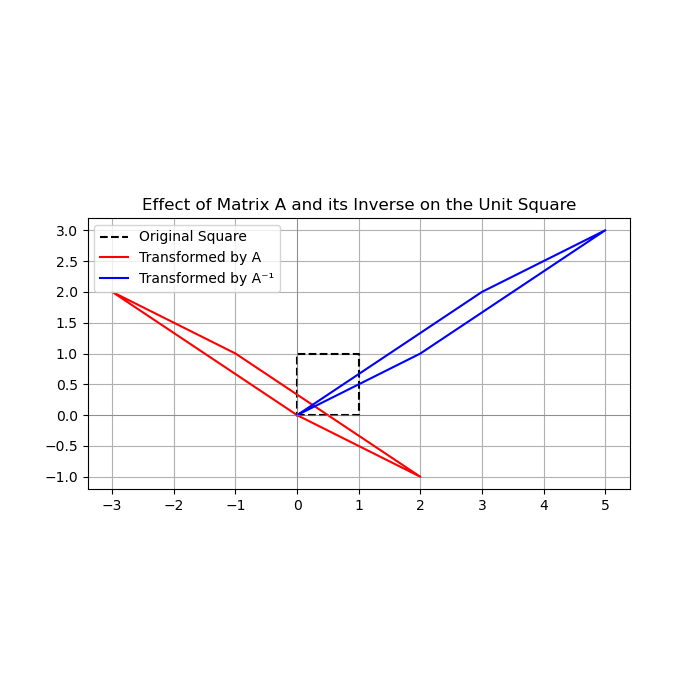
\includegraphics[width=\columnwidth, height=0.8\textheight, keepaspectratio]{Figs/fig11.png}     
\end{frame}

\begin{frame}[fragile]
\frametitle{C Code}
\begin{lstlisting}
#include <stdio.h>

int main() {
    float a, b, c, d;
    float det;
    
    // Input matrix
    printf("Enter the elements of 2x2 matrix:\n");
    scanf("%f %f", &a, &b);
    scanf("%f %f", &c, &d);
    \end{lstlisting}
\end{frame}

\begin{frame}[fragile]
\frametitle{C Code}
\begin{lstlisting}
    // Determinant
    det = a * d - b * c;

    if (det == 0) {
        printf("Inverse does not exist (determinant = 0)\n");
        return 0;
    }

    printf("Determinant = %.2f\n", det);
    \end{lstlisting}
\end{frame}

\begin{frame}[fragile]
\frametitle{C Code}
\begin{lstlisting}
    // Inverse formula:  1/det * [ d   -b ]
    
    //                             [ -c   a ]
    float inv_a =  d / det;
    float inv_b = -b / det;
    float inv_c = -c / det;
    float inv_d =  a / det;

    printf("Inverse matrix is:\n");
    printf("%.2f   %.2f\n", inv_a, inv_b);
    printf("%.2f   %.2f\n", inv_c, inv_d);

    return 0;
}
   \end{lstlisting}
\end{frame}

\begin{frame}[fragile]
\frametitle{Python and C Code}

\begin{lstlisting}

import ctypes
import numpy as np
import matplotlib.pyplot as plt

# Load compiled C library
# For Linux/Mac
lib = ctypes.CDLL('./libmatrix_inverse.so')
# For Windows:
# lib = ctypes.CDLL('matrix_inverse.dll')

# Define argument types
lib.inverse2x2.argtypes = [ctypes.POINTER(ctypes.c_double), ctypes.POINTER(ctypes.c_double)]
  \end{lstlisting}
\end{frame}

\begin{frame}[fragile]
\frametitle{Python and C Code}

\begin{lstlisting}

# Input matrix A = [[2, -3], [-1, 2]]
A = np.array([2.0, -3.0, -1.0, 2.0], dtype=np.float64)
A_inv = np.zeros(4, dtype=np.float64)

# Call C function to get inverse
lib.inverse2x2(A.ctypes.data_as(ctypes.POINTER(ctypes.c_double)),
               A_inv.ctypes.data_as(ctypes.POINTER(ctypes.c_double)))

# Reshape to 2x2 matrices
A_matrix = A.reshape(2, 2)
A_inv_matrix = A_inv.reshape(2, 2)
  \end{lstlisting}
\end{frame}

\begin{frame}[fragile]
\frametitle{Python and C Code}

\begin{lstlisting}

print("Original matrix A:")
print(A_matrix)
print("Inverse matrix A⁻¹ (from C):")
print(A_inv_matrix)

# Define the unit square
square = np.array([
    [0, 0],
    [1, 0],
    [1, 1],
    [0, 1],
    [0, 0]
])
  \end{lstlisting}
\end{frame}

\begin{frame}[fragile]
\frametitle{Python and C Code}

\begin{lstlisting}

# Apply transformations
square_A = square @ A_matrix.T
square_Ainv = square @ A_inv_matrix.T

# Plot
plt.figure(figsize=(8, 6))
plt.plot(square[:, 0], square[:, 1], 'k--', linewidth=1.5, label='Original Square')  # Black dashed
plt.plot(square_A[:, 0], square_A[:, 1], color='orange', linewidth=2.5, label='Transformed by A')  # Orange
plt.plot(square_Ainv[:, 0], square_Ainv[:, 1], color='green', linewidth=2.5, label='Transformed by A⁻¹')  # Green

# Optional: add markers to show square corners
plt.scatter(square[:, 0], square[:, 1], color='black')
plt.scatter(square_A[:, 0], square_A[:, 1], color='orange')
plt.scatter(square_Ainv[:, 0], square_Ainv[:, 1], color='green')
  \end{lstlisting}
\end{frame}

\begin{frame}[fragile]
\frametitle{Python and C Code}

\begin{lstlisting}

plt.grid(True)
plt.gca().set_aspect('equal', adjustable='box')
plt.title('Effect of Matrix A and its Inverse on the Unit Square')
plt.legend()
plt.xlabel("X-axis")
plt.ylabel("Y-axis")
plt.tight_layout()
plt.show()
  \end{lstlisting}
\end{frame}

\begin{frame}{Plot-Using by C and Python}
    \centering
    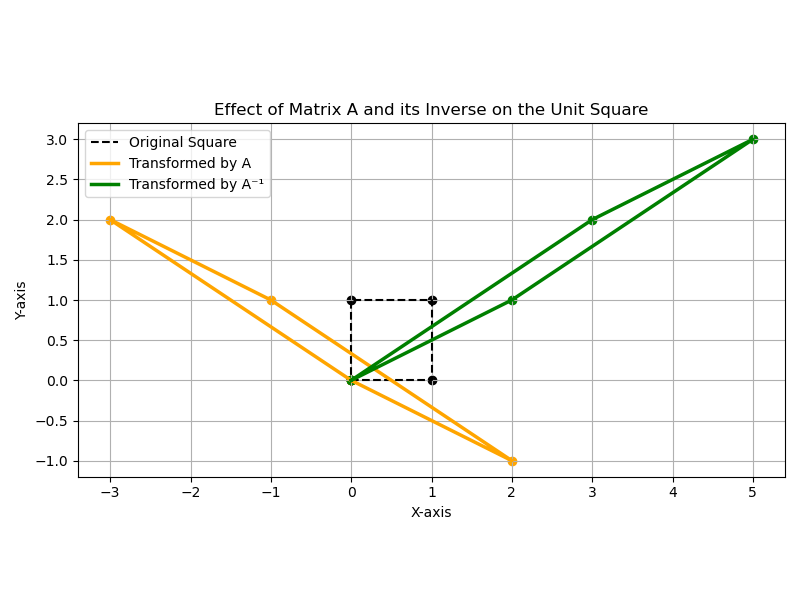
\includegraphics[width=\columnwidth, height=0.8\textheight, keepaspectratio]{Figs/fig11.1.png}     
\end{frame}
\end{document}
